\setlength{\parskip}{0.5em}
\noindent The primary function of the Traffic Pi is to use computer vision and object recognition to calculate the speed of a vehicle crossing the screen. We plan to mount an IR/Visible light camera along with a Raspberry Pi on the side of the road to allow regular citizens to perform their own traffic study. Our team has considered many risks such as environmental hazards and potential theft and plan to house our product inside a weather-proof, 3D-printed container.

\noindent With our product, we hope to find a solution to the massive costs of a standard traffic study—which includes hiring an engineer to lay cables to monitor the traffic on a street over a 24 hours period—with a computer vision-based product that will cost less and provide more information about vehicles passing through the designated study zone.

\noindent From a user's perspective, there will be very little setup required to begin conducting their own traffic study. Should the user need any help with configuration, our web page will provide adequate information to help walk the user through installing their Traffic Pi. Along with installation information, we will provide the user with an interface to manage any footage captured or data collected by the device. We will give the user the ability to see information such as how frequently vehicles passed through the area, how fast they were going, and even the actual vehicle that passed through the frame.

\noindent Alternatively, as a maintainer or administrator of the project, one should be able to provide a reliable service with the ability to self-update the Traffic Pi should the need for software management or troubleshooting arise. Our product will give administrators the ability to push any updates to the device software, force a restart of a device should a user need help with their device freezing or crashing, and general control by giving the user an interface to conduct low-level maintenance to the device. \par

\subsection{Features \& Functions}
\graphicspath{ {./images/} }
Traffic Pi main function is to detect and determine the speed of passing cars from a mantled raspberry pi (Figure 1) and document the information in a database. Detection will be processed through an IR/Visible light camera (Figure 2) that will be able to detect in both bright and dark environments. By user demand, the Traffic Pi will return documented data comprised of footage, speeds, time of day, and traffic activity. The data will be able to display through a user interface accessible on the customer’s personal computer including the ability to access the device through the cloud. Traffic Pi can also be able to connect to the internet to allow the ability to perform software updates. Traffic Pi’s main functionality is to detect and calculate the speed of passing cars, so the device will not function for the purpose of security nor will detect the activities outside of cars (i.e. pedestrians walking by). \newline\newline
Figure 1\newline
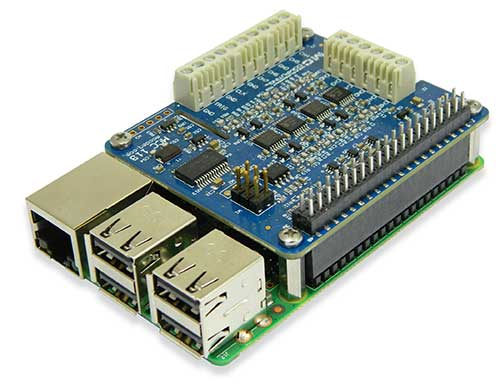
\includegraphics[width=14cm, height=10cm]{rasppi.jpg}\newline
Figure 2\newline
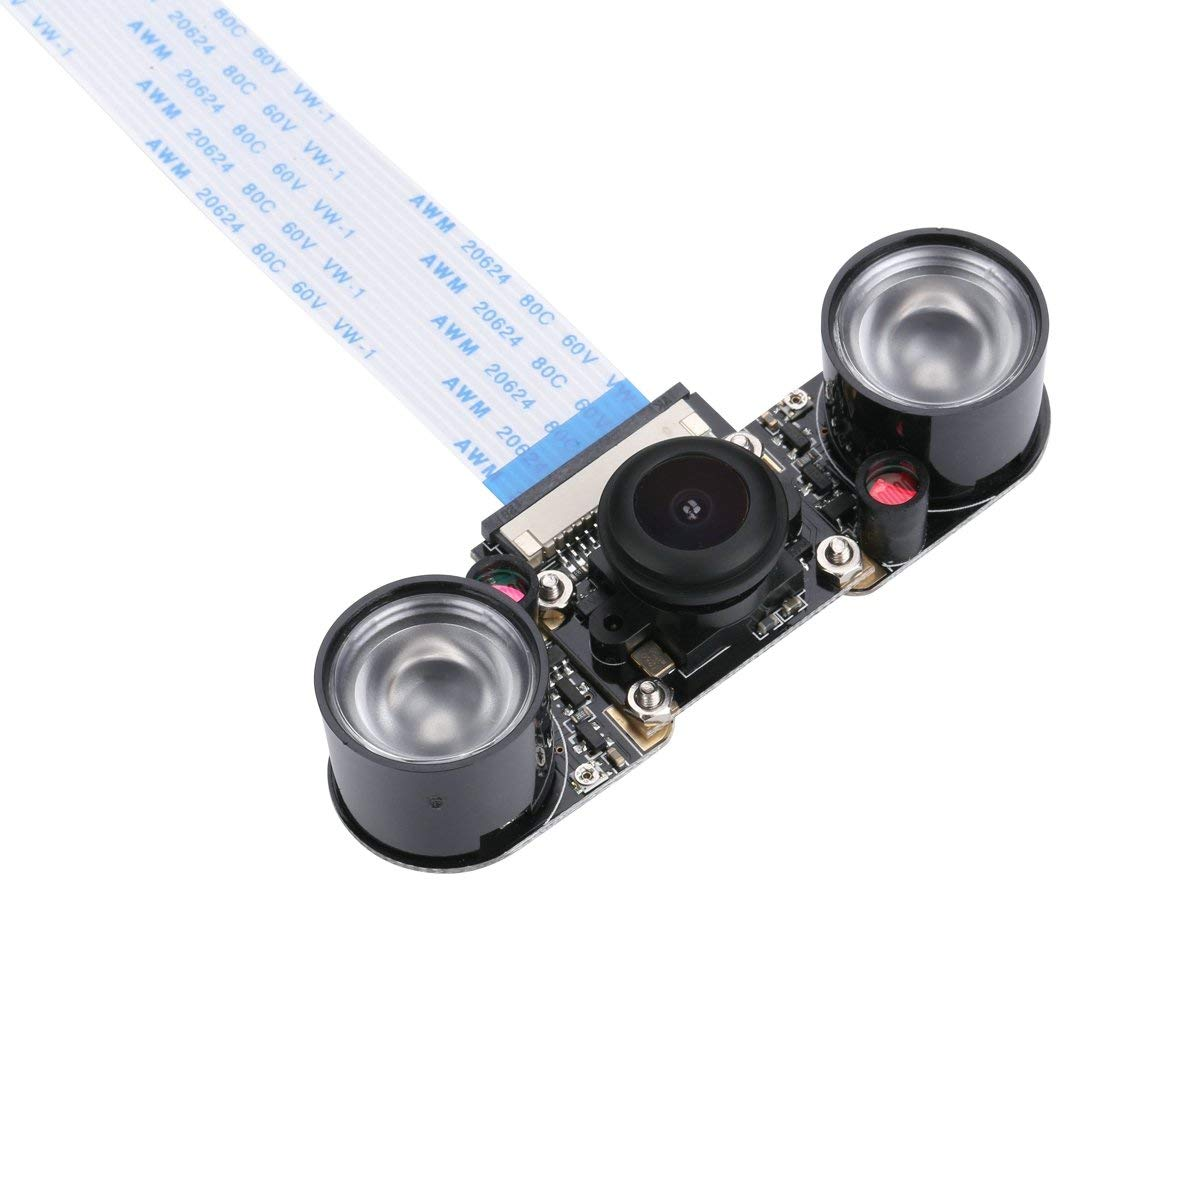
\includegraphics[width=14cm, height=10cm]{IR_camera.jpg}\newline

\subsection{External Inputs \& Outputs}
\begin{table}[h]
\centering
\resizebox{\textwidth}{!}{
\begin{tabular}{|l|l|l|}
\hline
 \textbf{Name} & \textbf{Description} & \textbf{Use}\\ \hline
 Arducam Noir  &  This will provide the video feed for the Traffic PI & Input \\ \hline
 Data Analytics & Captured data will be broken down and analyzed by a few metrics and uploaded to a cloud service & Output \\ \hline
 GUI & Data will be presented neatly to the user & Output \\ \hline
\end{tabular}}
\caption{Overview of External Inputs and Outputs}
\end{table}
\subsection{Product Interfaces}
\graphicspath{ {./images/} }
Homepage of the Traffic Pi website.\newline
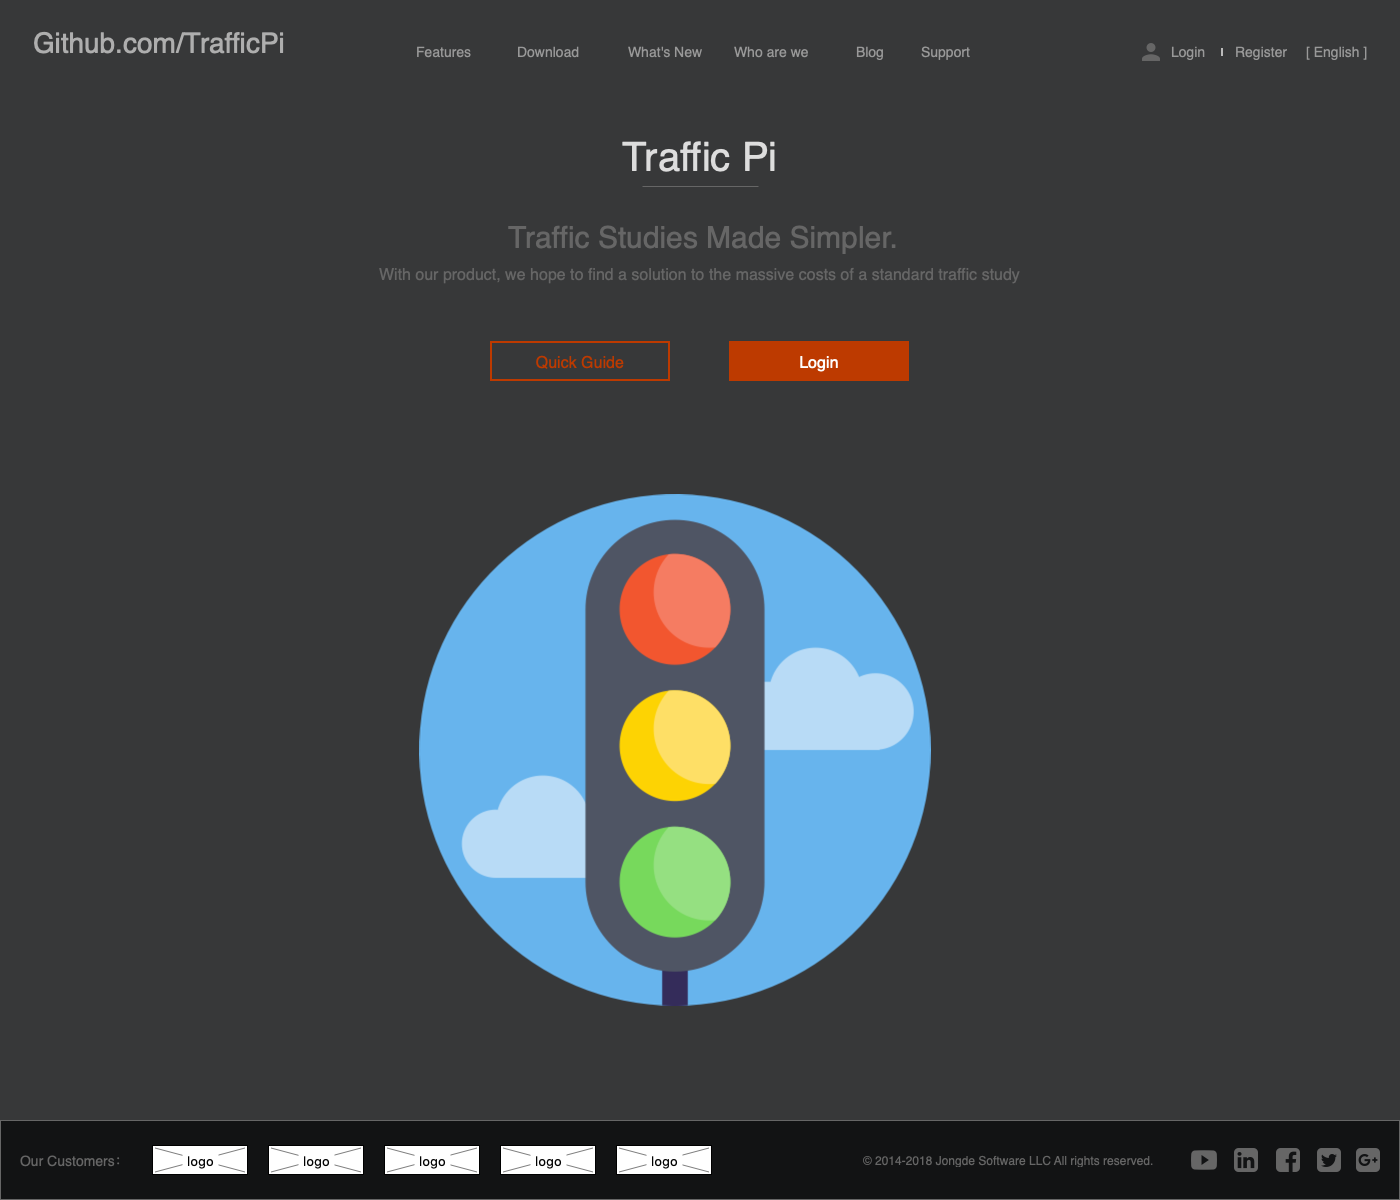
\includegraphics[width=14cm, height=10cm]{1-Home.png}\newline
Main dashboard page for end user.\newline
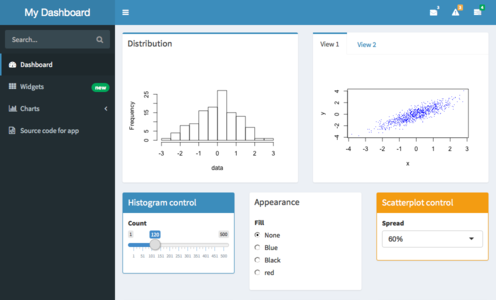
\includegraphics[width=14cm,height=10cm]{dashboard_1.png}\newline
Secondary dashboard page.\newline
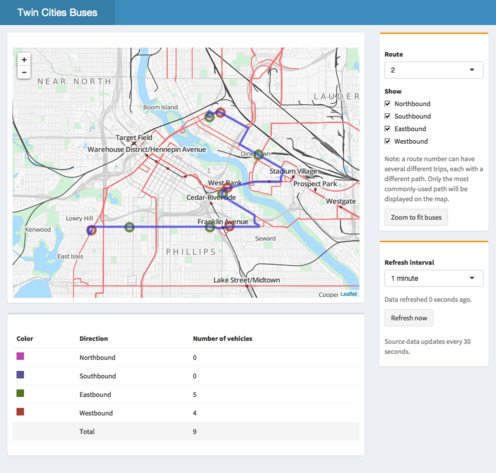
\includegraphics[width=14cm,height=10cm]{dashboard_2.png}\newline